	\chapter{Feature Engineering and Cross Validation}
	\section{Section FAQ}

	\resetquestioncounter{}
	\begin{qanda}
		\begin{question}
How do False-negative and False positive values change in the confusion matrix? Are they inversely related?
		\end{question}

		\begin{answer}
When we build a model and our target variable has a binary category and then we look at the confusion matrix. There are four elements:
		\begin{code}[\codenumbering]{}
			\codeitemnonumber True Positive (observed=1, predicted=1)
			\codeitemnonumber False Positive (observed=0, predicted=1)
			\codeitemnonumber True Negative (observed=0, predicted=0)
			\codeitemnonumber False Negative (observed=1, predicted=0)
		\end{code}
The default threshold is 0.5. We change the threshold when we want to decrease or increase the number of false positives or false negatives.

Consider a credit card default problem for a bank. So if the model predicts that a person will default and the person doesn't then the bank might lose a potential customer but if the model predicts a customer would not default and he does, in the scenarios company would lose money. So the bank would want this number to be small.

Assuming defaulter to be 1 and non-defaulter to be 0 then the company would want lower False negatives. So we will try to build the model with a lower threshold so more people will be predicted as defaulters.

As you will try to decrease FN, FP will increase because of the values which were previously predicted as TN might change to FP, that is why prof must have said about the inverse relationship. So if we try to decrease FN via changing threshold all values in the confusion matrix change and FN will decrease but FP will increase.
		\end{answer}
	\end{qanda}

	\begin{qanda}
		\begin{question}
How to deal with outliers?
		\end{question}

		\begin{answer}
How to treat outliers is a very tricky topic, it mainly depends on the problem statement. Sometimes we can't even remove outliers or treat them because that's just the way data is and should be kept like that for analysis.

Let us consider an example of a bank.  In a bank, account balance might have high outliers as few people will have a high amount in their accounts, but should we be treating this value or removing it? So I think here we have to consider that in practical life situations we cannot remove these accounts and if we replace them with any other value that will make the data biased.

So the best option would be thinking with respect to the problem statement. If the problem statement is: Who is more likely to do a credit card default then I think we can remove people with a high balance in their account as they are less likely to default. In another case, if the problem statement is: Who is going to take a home loan then also I think we can remove outliers but if our problem statement is about business loans then we have to consider these outliers having high balance as they might take a loan for their business.

All the above judgments should be made by doing the necessary EDA on the data set to figure out the relationship of balance with the target (credit card default, home loan, business loan, etc.). None of the conclusions should come without the data supporting them.

Replacing the outliers is done when outliers are few in number and we think that this would be because of the wrong imputation. So we remove these outliers and treat them as missing data.
		\end{answer}
	\end{qanda}

	\begin{qanda}
		\begin{question}
Why can't we use the ROC\_AUC score in case of a skewed data set?
		\end{question}

		\begin{answer}
This is because a small number of correct or incorrect predictions can result in a large change in the ROC Curve or ROC AUC score, that is why precision and recall are preferred more in case of skewed data.
		\end{answer}
	\end{qanda}

	\begin{qanda}
		\begin{question}
What are imbalanced data sets?
		\end{question}

		\begin{answer}
Imbalanced data sets are those where there is a severe skew in the class distribution, such as 1:100 or 1:1000 examples in the minority class to the majority class.

This bias in the training data set can influence many machine learning algorithms, leading some to ignore the minority class entirely. This is a problem as it is typically the minority class on which predictions are most important.
		\end{answer}
	\end{qanda}

	\begin{qanda}
		\begin{question}
What are the techniques to handle imbalanced data sets?
		\end{question}

		\begin{answer}
One approach to addressing the problem of class imbalance is to randomly re-sample the training data set. The two main approaches to randomly resampling an imbalanced data set are to delete examples from the majority class, called under sampling, and to duplicate examples from the minority class, called over sampling.
		\end{answer}
	\end{qanda}

	\begin{qanda}
		\begin{question}
What is Cross-Validation?
		\end{question}

		\begin{answer}
Cross-Validation is a very useful technique for assessing the performance of machine learning models. It helps in knowing how the machine learning model would generalize to an independent data set. You want to use this technique to estimate how accurate the predictions your model will give in practice.
		\end{answer}
	\end{qanda}

	\begin{qanda}
		\begin{question}
What are polynomial Features and when to use them? why do we need additional features, which are going to be derived from existing features? Is it not the case of over fitting?
		\end{question}

		\begin{answer}
Polynomial features are used to convert features to a higher degree.

If there are 2 features $[a, b]$, then degree-2 polynomial features are $[1, a, b, a^2, ab, b^2]$.

This is a pre-processing technique after converting to a higher degree we can use the new features for any algorithm like a ridge, lasso, logistic, decision tree, etc.  We use polynomial features when the relationship between the target variable and independent variables is nonlinear.

One way to check whether a data set is nonlinear is negative r2score. R2score will be negative when the relationship between the target variable and independent variables is nonlinear. Then we introduce the polynomial features to check for higher degree terms.
Polynomial features not necessarily increase over fitting, it increases redundant columns but not over fitting. So we remove all the correlated features when we want to check which features are driving the model if the sole aim of the model is a higher score then these redundant columns don't hurt.

We can use polynomial features to check for interaction between the features as well by interaction\_only=True.
		\end{answer}
	\end{qanda}

	\begin{qanda}
		\begin{question}
How K-Fold Cross-validation works?
		\end{question}

		\begin{answer}Here is the thing:
		\begin{bulletedlist}
			\item If k-fold cross-validation is used to optimize the model parameters, the training set is split into k parts.
			\item Training happens k times, each time leaving out a different part of the training set.
			\item Typically, the error of these k-models is averaged.
			\item This is done for each of the model parameters to be tested, and the model with the lowest cross-validated and validation error is chosen.
			\item The test set has not been used so far.
			\item Only at the very end, the test set is used to test the performance of the (optimized) model.
		\end{bulletedlist}
		\begin{code}[\codenumbering]{}
			\codeitemnonumber \# example: k-fold cross validation for hyperparameter optimization (k=3)
			\codeitemnonumber original data split into training and test set:
			\codeitemnonumber |---------------- train ---------------------|         |--- test ---|
			\codeitemnonumber
			\codeitemnonumber cross-validation: test set is not used, error is calculated from
			\codeitemnonumber validation set (k-times) and averaged:
			\codeitemnonumber
			\codeitemnonumber |---- train ------------------|- validation -|         |--- test ---|
			\codeitemnonumber |---- train ---|- validation -|---- train ---|         |--- test ---|
			\codeitemnonumber |- validation -|----------- train -----------|         |--- test ---|
			\codeitemnonumber
			\codeitemnonumber final measure of model performance: model is trained on all training data
			\codeitemnonumber and the error is calculated from test set:
			\codeitemnonumber
			\codeitemnonumber |---------------- train ---------------------|--- test ---|
		\end{code}

\begin{bulletedlist}
	\item In some cases, k-fold cross-validation is used on the entire data set if no parameter optimization is needed (this is rare, but it happens).
	\item In this case, there would not be a validation set and the k parts are used as a test set one by one.
	\item The error of each of these k tests is typically averaged.
\end{bulletedlist}
		\begin{code}[\codenumbering]{}
			\codeitemnonumber \# example: k-fold cross validation
			\codeitemnonumber
			\codeitemnonumber |----- test -----|------------ train --------------|
			\codeitemnonumber |----- train ----|----- test -----|----- train ----|
			\codeitemnonumber |------------ train --------------|----- test -----|
		\end{code}
		\end{answer}
	\end{qanda}

	\begin{qanda}
		\begin{question}
Should we apply the transformations AFTER splitting the data into train/test/validation to prevent data leaks?
		\end{question}

		\begin{answer}Yes. Data preparation must be fit on the training data set only. That is, any coefficients or models prepared for the data preparation process must only use rows of data in the training data set.

Once fit, the data preparation algorithms or models can then be applied to the training data set, and the test data set.
			\begin{numberedlist}
				\item Split Data.
				\item Fit Data Preparation on Training data set.
				\item Apply Data Preparation to Train and Test data sets.
				\item Evaluate Models.\end{numberedlist}\end{answer}\end{qanda}


	\begin{qanda}
		\begin{question}
Why do we need to do one-hot encoding after splitting the data even though one-hot encoding doesn't lead to data leakage?
		\end{question}

		\begin{answer}
We might do one hot encoding after splitting data if we have missing values in categorical columns as we can't do one-hot encoding for variables with missing values
And missing value imputation leads to data leakage, so should be done after splitting the data.
		\end{answer}
	\end{qanda}


	\section{Need for cross-validation}
	\begin{bulletedlist}
		\item We wish to know how well a Machine Learning model is likely to perform in production
		\item To estimate the model production score, we divide the data into 3 parts.
		\item Usually the available data is not sufficient to split into training, test and validation sets and expect them to represent the universe.
		\item As a result, the performance on training data may not be a good estimate of the performance in the universe.
		\item Using cross validation techniques can help us achieve a generalized model performance.
		\item This technique is also very useful in the absence of large data sets.
	\end{bulletedlist}

	\section{Cross Validation}
	\begin{bulletedlist}
		\item Cross-validation divides data into k folds.
		\item k-1 folds are used for training and the kth fold is used for testing purposes.
		\item The process is repeated k times.
		\item k different scores will be obtained.
		\item The final model performance is calculated by taking the average of k scores.
		\item We can also calculate the standard deviation of those scores and using that we can say that with 95\% confidence our model's performance will belong to:
	\end{bulletedlist}
%(avg - 2*std. dev., avg + 2*std dev)
	\begin{equation}
%		\left(\samplemean - 2*\samplestandarddeviation, \samplemean + 2*\samplestandarddeviation\right)
		\left(\samplemean - 2*\samplestandarddeviation{}, \samplemean + 2*\samplestandarddeviation{}\right)
	\end{equation}
	\begin{figure}[h]
		\centering
		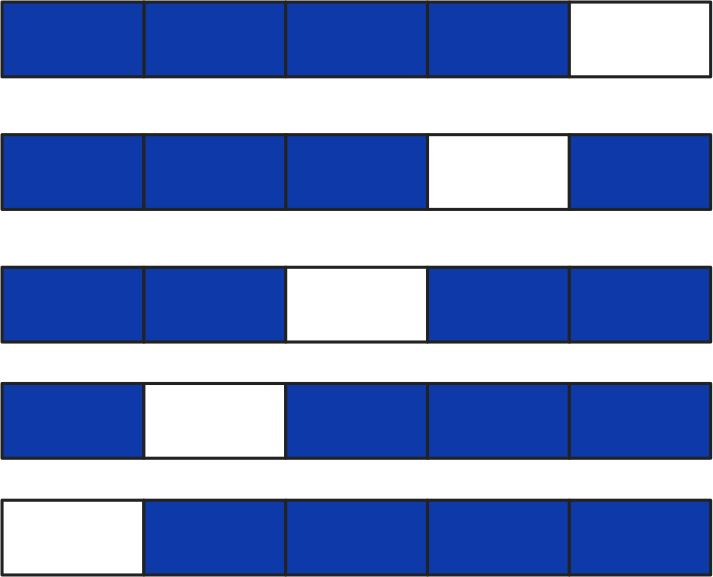
\includegraphics[height=1.5in]{crossvalidation}
		\caption[Cross validation]{Cross validation.}
		\label{fig:normaldistrution}
	\end{figure}


	\section{Choosing the Value of K}
	\begin{bulletedlist}
		\item k is an integer.
		\item Minimum value of k has to be 2, there will be two iterations in this case.
		\item Max value of k can be the number of data points, this is also known as Leave One Out Cross Validation or LOOCV
		\item Whatever the value of k chosen, the resulting training and test data should be representative of the unseen data as much as possible.
		\item There is no formula to decide the k but k = 10 is usually considered good.
		\item Too large a k, means less variance across the training sets thus limit the model differences across iterations.
		\item For a sample size of n, And k = p, Number Of Records (r) per fold = n/p.
	\end{bulletedlist}


	\section{Over Sampling and Under Sampling}
Over sampling and under sampling rely on having a few features that can differentiate between the feature that is being predicted.  If no features can differentiate between out the predicted class, prediction is difficult in general.

We can handle the imbalanced data set cases to minimize the Type II errors by balancing the class representations.  To balance the classes we can either decrease the frequency of the majority class or increase the frequency of the minority class.
	\begin{figure}[h]
		\centering
		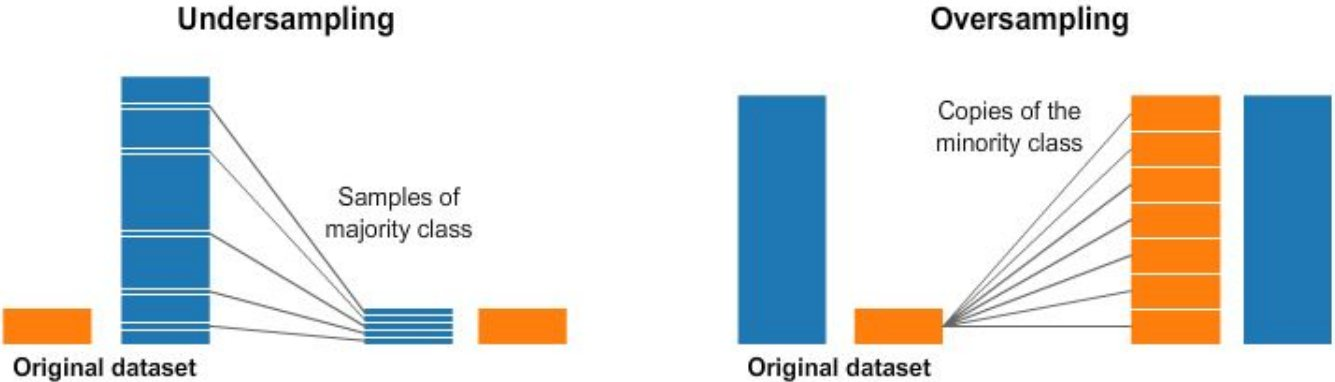
\includegraphics[width=5.0in]{overandundersampling}
		\caption[Over and under sampling]{Over and under sampling.}
		\label{fig:overandundersampling}
	\end{figure}

The simplest implementation of over-sampling is to duplicate random records from the minority class, which can cause over fitting.

In under-sampling, the simplest technique involves removing random records from the majority class, which can cause loss of information.

	\subsection{SMOTE}
SMOTE (Synthetic Minority Oversampling TEchnique)
	\begin{bulletedlist}
		\item Syntheses elements for the minority class, based on those that already exist.
		\item It works randomly picking a point from the minority class and computing the k-nearest neighbors (KNN) for this point.
		\item Synthetic points are added between the chosen point and its neighbors.
	\end{bulletedlist}


	\section{Linear Regression Regularization}

When we have too many parameters and exposed to curse of dimensionality, we resort to dimensionality reduction techniques such as transforming to PCA and eliminating the PCA with least magnitude of eigenvalues. This can be a laborious process before we find the right number principal components. Instead, we can employ the shrinkage methods.  Shrinkage methods attempt to shrink the coefficients of the attributes and lead us towards simpler yet effective models. The two shrinkage methods are:

Why should we be interested in shrinking the coefficients? How does it help?  When we have large number of dimensions and few data points, the models are likely to become complex, over fit and prone to variance errors. When you print out the coefficients of the attributes of such complex model, you will notice that the magnitude of the different coefficients become large.

Large coefficients indicate a case where for a unit change in the input variable, the magnitude of change in the target column is very large.

	\begin{figure}[tbh]
		\centering
		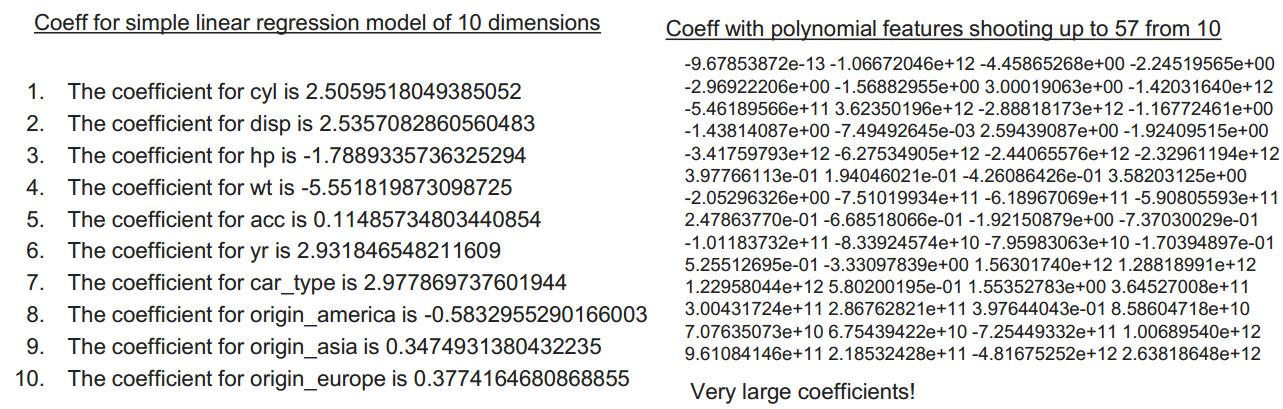
\includegraphics[width=\textwidth]{modelcoefficients}
		\caption[Model coefficients]{Model coefficients.}
		\label{fig:modelcoefficients}
	\end{figure}

	\begin{bulletedlist}
		\item Curse of dimensionality results in large magnitude coefficients which results in a complex undulated surface / model.
		\item This complex surface has the data points occupying the peaks and the valleys.
		\item The model gives near 100\% accuracy in training but poor result in testing and the testing scores also vary a lot from one sample to another.
		\item The model is supposed to have absorbed the noise in the data distribution!
		\item Large magnitudes of the coefficient give the least SSE and at times SSE = 0! A model that fits the training set 100\%!
		\item Such models do not generalize.
		\item Very large values of the penalty term leads to under fitting (model has been smoothed too much).
	\end{bulletedlist}

	\subsection{Ridge Regression}
	\begin{bulletedlist}
		\item Ridge regression is similar to the linear regression where the objective is to find the best fit surface. The difference is in the way the best coefficients are found. Unlike linear regression where the optimization function is \gls{sse}, here it is slightly different (see \figurename~\ref{fig:linearversusridgeregression})
		\item The term $\lambda$ is a penalty term used to penalize large magnitude coefficients, $\beta_j$.  When it is set to a high number, coefficients are suppressed significantly.  When it is set to 0, the cost function becomes the same as the linear regression cost function.
		\item The extra term works to suppress peaks and valleys (the sharp points of the fitted equation) and create a smoother surface.
		\item The penalty term is the sum of squared values of the coefficients.
	\end{bulletedlist}

	\begin{figure}[tbh]
		\centering
		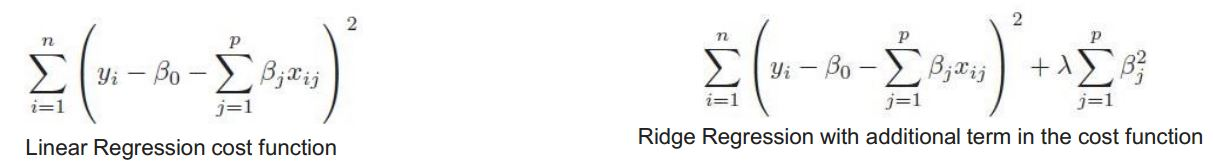
\includegraphics[width=\textwidth]{linearversusridgeregression}
		\caption[Linear versus ridge regression]{Linear versus ridge regression.}
		\label{fig:linearversusridgeregression}
	\end{figure}

	\begin{bulletedlist}
		\item In Ridge Regression, the algorithm while trying to find the best combination of coefficients which minimize the SSE on the training data, is constrained by the penalty term.
		\item The penalty term is akin to cost of magnitude of the coefficients. Higher the magnitude, more the cost. Thus to minimize the cost, the coefficient are suppressed
		\item Thus the resulting surface tends to be relatively much more smoother than the unconstrained surface. This means we have settled for a model which will make errors in the
training data.
		\item This is fine as long as the errors can be attributed to the random fluctuations i.e.\ because the model does not absorb the random fluctuations in the data.
		\item Such model will perform equally well on unseen data i.e.\ test data. The model will generalize better than the complex model.
	\end{bulletedlist}

	\subsection{Lasso Regression}

	\begin{bulletedlist}
		\item Lasso Regression is similar to the Ridge regression with a difference in the penalty term. Unlike Ridge, the penalty term here is raised to power 1. Also known as L1 norm.
		\item The term continues to be the input parameter which will decide how high penalties would be for the coefficients. Larger the value more diminished the coefficients will be.
		\item Unlike Ridge regression, where the coefficients are driven towards zero but may not become zero, Lasso Regression penalty process will make many of the coefficients 0. In other words, literally drop the dimensions.  This is effectively automatic feature selection.
		\item Penalty adds up magnitude of coefficients instead of the square of the coefficients that ridge regression does.
	\end{bulletedlist}

	\begin{equation}
		\sum^M_{i=1} \left(y_i - \sum^P_{j=0} w_j \times x_{ij} \right)^2  +  \lambda \sum^P_{j=0} \left| w_j \right|
	\end{equation}

	\subsection{Comparing Ridge and Lasso}
To compare the Ridge and Lasso, let us first transform our error function (which is a quadratic / convex function) into a contour graph.

	\begin{bulletedlist}
		\item Every ring on the error function represents a combination of coefficients (m1 and m2 in the image) which result in same quantum of error i.e.\ SSE.
		\item Let us convert that to a 2D contour plot.  In the contour plot, every ring represents one quantum of error.
		\item The innermost ring / bull's eye is the combination of the coefficients that gives the lease SSE.
	\end{bulletedlist}

	\begin{figure}[tbh]
		\centering
		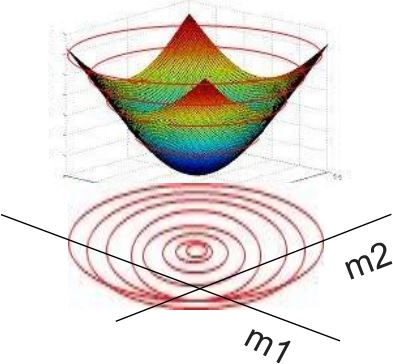
\includegraphics[width=2.0in]{ridgeversuslasso1}
		\caption[Ridge versus Lasso regression]{Ridge versus Lasso regression.}
		\label{fig:ridgeversuslasso1}
	\end{figure} 